\section{FUNDAMENTAÇÃO TEÓRICA}

    \ipar Nesta seção são apresentados os conceitos e modelos matemáticos que fundamentam o desenvolvimento deste trabalho. Para elaborar a fundamentação destes conceitos, são considerados três aspectos: modelos de risco e retorno de ativos financeiros, métodos e parâmetros de otimização de portfólio e estruturas de redes neurais. Estes aspectos são abordados considerando a aplicação do índice Sharpe nas pesquisas relacionadas ao tema de pesquisa deste trabalho.
    
    \ipar A avaliação destes aspectos passa por uma revisão sistemática da literatura, que é apresentada na seção \ref{sec:revisao_sistematica}. A seção \ref{sec:retorno} apresenta os modelos de risco e retorno de ativos financeiros, a seção \ref{sec:otimizacao} apresenta os modelos de otimização de portfólio e a seção \ref{sec:redesneurais} apresenta as estruturas de redes neurais.

    \subsection{REVISÃO SISTEMÁTICA DA LITERATURA}
        \label{sec:revisao_sistematica}

        \ipar A revisão sistemática da literatura busca identificar as principais referências relacio-nadas ao tema, seguindo um protocolo orientado a este objetivo. As etapas para um protocolo de revisão sistemática são: definição da questão de pesquisa, definição dos critérios de seleção, busca e seleção dos estudos, extração dos dados e análise dos resultados. Pode-se utilizar métodos matemáticos e estatísticos para auxiliar na análise dos resultados, como a análise bibliométrica \cite{yu2018bibliometric}. 
        
        \ipar \citeonline{milhomem2020analysis} apresenta uma revisão sistemática da literatura sobre otimi-zação de carteiras dado a dual de risco e retorno para avaliação de questões sobre métodos, técnicas e ferramentas para otimização, quais restrições reais são aplicadas, e que tipo de análise financeira foi realizada na pesquisa, além dos programas utilizados. Estendo a esta pesquisa, as etapas desenvolvidas neste trabalho, seguem a estrutura que são apresentadas no quadro \ref{quadro:protocolo_revisao_sistematica}.

        \begin{quadro}[htbp]
            \centering
            \caption{Protocolo de revisão sistemática da literatura}
            \label{quadro:protocolo_revisao_sistematica}
            \begin{tabular}{p{0.25\linewidth}p{0.65\linewidth}}
                % quadro
                \hline
                \textbf{Estágio} & \textbf{Descrição} \\
                \hline \hline
                \textbf{Tema central:} & Redes neurais aplicados a otimização de carteiras de investimentos. \\ \hline
                \textbf{Estrutura conceitual:} & O modelo de Markowitz contribuiu para diversos outros estudos explorarem métodos para a otimização de carteiras. O objetivo desta revisão é identificar os métodos mais relevantes para três aspectos: modelos de risco e retorno de ativos financeiros, métodos e restrições para otimização de portfólio e estruturas de redes neurais aplicado ao índice Sharpe. \\ \hline
                \textbf{Escopo:} & A revisão será realizada considerando os artigos publicados entre 2019 a 2023, com objetivo de encontrar os documentos mais relevantes publicados nos últimos 5 anos. \\ \hline
                \textbf{Corrente teórica: } & Otimização de portfólio, redes neurais e índice Sharpe. \\ \hline
                \textbf{Idioma:} & Inglês. \\ \hline
                \multirow{3}{*}{\textbf{Questões de pesquisa:}} & Questão 1: Quais são os métodos utilizados para avaliação de risco e retorno de ativos financeiros? \\
                & Questão 2: Quais são os métodos e restrições reais aplicados para otimização de portfólio? \\
                & Questão 3: Quais estruturas de redes neurais são aplicadas ao índice Sharpe? \\ \hline
                \textbf{Critérios de inclusão:} & Título, palavras chaves ou resumos que apresentam relação com otimização de portfólio e estruturas de redes neurais aplicado ao índice Sharpe. \\ \hline
                \textbf{Critérios de exclusão:} & Artigos duplicados, ou não públicos e sem acesso via CAPES. \\ \hline
                \multirow{4}{*}{\textbf{\textbf{Termos de busca:}}} & Pesquisa 1: \textit{Portfolio optimization} \& \textit{Neural Network}, \\
                & Pesquisa 1: \textit{Portfolio optimization} \& \textit{Machine Learning}, \\
                & Pesquisa 3: \textit{Portfolio optimization} \& \textit{Deep Learning},\\
                \textbf{Fontes de pesquisa:} & \textit{Web of Science}. \\ \hline
            \end{tabular}
            \par \footnotesize Fonte: próprio autor. % Fonte: \citeonline{Autor_bibtex}.
        \end{quadro}

        \ipar Como resultado do processo de revisão sistemática, de uma lista de 577 artigos da base de dados, foram identificados 48 que atendem aos critérios de inclusão. Para obter uma visão macro sobre os artigos, foi realizada uma análise bibliométrica com uso da ferramenta bibliometrix \cite{aria2017bibliometrix}. Inicialmente, para observar as referências mais citadas em conjunto, foi realizada uma análise de co-citação. A figura \ref{fig:co_citacao} apresenta o mapa de co-citação dos artigos.

        \begin{figure}[htbp]
            \centering
            \caption{Mapa de co-citação dos artigos}
            \label{fig:co_citacao}
            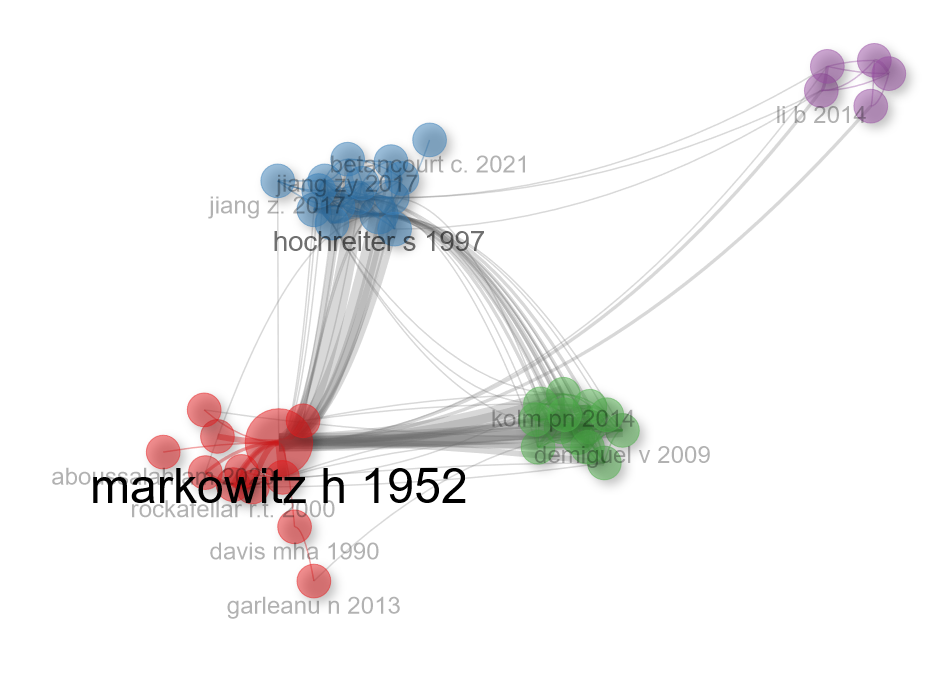
\includegraphics[width=0.9\textwidth]{./imagens/cocitation_network.png}
            \par \footnotesize Fonte: próprio autor.
        \end{figure}

        \ipar Dentre os artigos mais citados em conjunto, observa-se que \citeonline{markowitz1952portfolio} é a referência que apresenta maior número de conexões entre os citações. Isto ocorre, pois a fundamenta-ção da teoria de seleção de portfólio tem como base este trabalho. É possível observar que há a formação de alguns grupos de co-citação. Um grupo contém os documentos de \citeonline{kolm2014years}, que realiza uma revisão ampla de 60 anos da teoria de otimização de portfólio, em conjunto com \citeonline{demiguel2009optimal}, que compara resultados de portfólio ótimos com modelos uniformes $1/N$. Outro grupo, contém o documento de \citeonline{hochreiter1997long}, que apresenta a estrutura de redes neurais recorrentes \acrshort{LSTM}.
        
        \ipar A relação das referências com os documentos selecionados é avaliado na figura \ref{fig:tree_field_plot}. Nesta figura é realizado o filtro das 10 referências mais citadas pelos artigos selecionados, e quais palavras dos títulos e palavras chaves são mais recorrentes e alinhadas com as referências.

        \begin{figure}[htbp]
            \centering
            \caption{Relação das referências com os títulos dos documentos selecionados}
            \label{fig:tree_field_plot}
            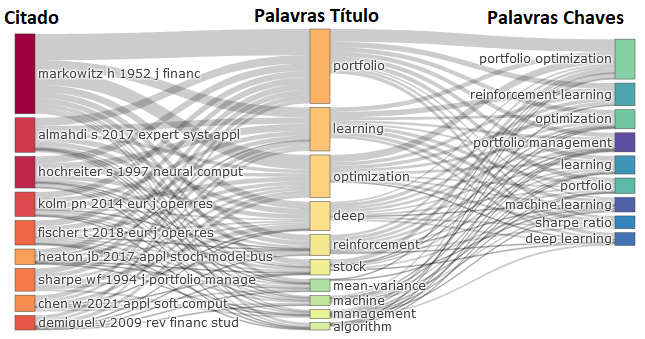
\includegraphics[width=.8\textwidth]{./imagens/tree_field_plot.png}
            \par \footnotesize Fonte: próprio autor.
        \end{figure}

        \ipar Pela figura \ref{fig:tree_field_plot}, nota-se que as principais referências estão relacionadas com o tema de otimização de portfólio, com aprendizagem de máquina e com o índice Sharpe. Portanto, os artigos selecionados estão alinhados com o tema de pesquisa deste trabalho.

        \ipar Para uma melhor compreensão das principais referencias, artigos com 5 ou mais citações pelos documentos selecionados são descritos no quadro \ref{quadro:citados}.


        \begin{quadro}[htbp]
            \centering
            \caption{Referências mais citadas pelos documentos selecionados}
            \label{quadro:citados}
            \begin{tabular}{p{0.25\linewidth}cp{0.55\linewidth}}
                \hline 
                Referência citada & Citações & Visão Geral \\ \hline \hline
                \citeonline{markowitz1952portfolio} & 31 & Teoria Moderna de Portfólio. \\ \hline
                \citeonline{almahdi2017adaptive} & 8 & Alocação de carteira utilizando aprendizagem por reforço recorrente com máximo \textit{drawdown}. \\ \hline
                \citeonline{hochreiter1997long} & 8 & Redes neurais recorrentes \acrshort{LSTM}. \\ \hline
                \citeonline{kolm2014years} & 8 & Revisão de 60 anos da teoria de otimização de portfólio. \\ \hline
                \citeonline{demiguel2009optimal} & 7 & Comparação de portfólio ótimo com modelo uniforme $1/N$. \\ \hline
                \citeonline{fischer2018deep} & 7 & Previsão de movimento de mercado com LSTM aplicado a grande dimensionalidade. \\ \hline
                \citeonline{sharpe1994sharpe} & 7 & Índice de Sharpe. \\ \hline
                \citeonline{chen2021mean} & 6 & Combina método de predição de aprendizagem de máquina XGBoost com modelo de média-variância para seleção de carteiras. \\ \hline
                \citeonline{heaton2017deep} & 6 & Revisão sobre o arcabouço de otimização de portfólio utilizando aprendizagem profunda. \\ \hline
                \citeonline{moody1998performance} & 6 & Aprendizagem por reforço com aplicação do índice Sharpe com custos de transação para construção de carteiras. \\ \hline
                \citeonline{wang2020portfolio} & 6 & Combinação de \acrshort{LSTM} com modelo de média-variância para construção de carteira ótima. \\ \hline
                \citeonline{artzner1999coherent} & 5 & Avaliação sobre a compreensão, aceitação e percepção de risco. \\ \hline
                \citeonline{chen2016xgboost} & 5 & Método de aprendizagem de máquina de larga escala XGBoost. \\ \hline
                \citeonline{chong2017deep} & 5 & Modelo de aprendizagem profunda de atributos para previsão de mercado de ações. \\ \hline
                \citeonline{deng2016deep} & 5 & Modelo de aprendizagem profunda para identificação de atributos combinado com aprendizagem com reforço para ação de investimentos. \\ \hline
                \citeonline{kingma2015adam} & 5 & Algoritmo de otimização Adam aplicado a redes neurais. \\ \hline
                \citeonline{mnih2015human} & 5 & Aprendizagem por reforço profundo aplicado a jogos Atari. \\ \hline
                \citeonline{rockafellar2000optimization} & 5 & Valor em risco condicional \acrshort{CVaR}. \\ \hline
                \citeonline{sutton2018reinforcement} & 5 & Introdução sobre aprendizagem por reforço. \\ \hline
            \end{tabular}
            \par \footnotesize Fonte: próprio autor.
        \end{quadro}

        \ipar A partir da análise do quadro \ref{quadro:citados}, pode-se identificar algumas temáticas principais, modelos de otimização de carteiras, modelos de aprendizagem de máquina, e combinação de ambos. Os principais modelos de otimização são o de média-variância de \citeonline{markowitz1952portfolio}, maximização do índice Sharpe \cite{sharpe1994sharpe}, e o de valor em risco condicional de  \citeonline{rockafellar2000optimization}. Os modelos de aprendizagem de máquina mais citados são \acrshort{LSTM} de \citeonline{hochreiter1997long}, XGBoost de \citeonline{chen2016xgboost} e aprendizagem por reforço para finanças de \citeonline{moody1998performance} combinados com redes neurais \cite{mnih2015human}.

        \subsubsection{Métodos de risco e retorno de ativos}

            \ipar Avaliando o conteúdo dos estudos selecionados quanto a quais são os métodos mais utilizados para risco e retorno de ativos, foi elaborado o quadro \ref{quadro:metodos_risco_retorno} que apresenta os métodos por algumas referências. Quando não realizada a otimização diretamente pela rede neural, aplica-se os seguintes métodos de risco e retorno nas séries temporais para o cálculo das carteiras.

            \begin{quadro}[htbp]
                \centering
                \caption{Métodos de risco e retorno de ativos}
                \label{quadro:metodos_risco_retorno}
                \begin{tabular}{lll}
                    \hline
                    Referência & Risco e Retorno \\ \hline \hline
                    \citeonline{yu2019fusing} & \acrshort{ARMA}-\acrshort{GARCH} \\
                    \citeonline{ta2020portfolio} & Média e Covariância \\
                    \citeonline{yu2020neural} & \acrshort{GARCH} \\
                    \citeonline{vukovic2020neural} & Média Móvel \\
                    \citeonline{zhu2020portfolio} & Média Móvel Exponencial \\
                    \citeonline{lee2021learning} & Média Móvel \\ 
                    \citeonline{leow2021robo} & Média Móvel Exponencial \\
                    \citeonline{liang2021portfolio} & Média Móvel Exponencial \\
                    \citeonline{chaweewanchon2022markowitz} & Média, Mediana \\
                    \citeonline{zhou2023twostage} & Média Móvel \\
                    \hline
                    \end{tabular}
                \par \footnotesize Fonte: próprio autor.
            \end{quadro}

            \ipar Assim, pode-se observar que os métodos mais utilizados são a média móvel exponencial, média móvel, média e covariância, e \acrshort{GARCH} para a consideração de risco e retorno de ativos como forma de entrada para otimização. A média e covariância representa o retorno médio da série temporal e a covariância a relação do desvio padrão do ativo e correlação entre este e os demais \cite{markowitz1952portfolio}. A média móvel é um método de suavização de séries temporais. A média móvel exponencial é um método de suavização de séries temporais, que atribui pesos decrescentes para os dados mais antigos, e pesos crescentes para os dados mais recentes \cite{winters1960ewm}. O \acrshort{GARCH} é um modelo de previsão de volatilidade de séries temporais, que considera a volatilidade condicional, ou seja, a volatilidade de um período é calculada em função da volatilidade do período anterior \cite{bollerslev1986generalized}. Portanto, neste trabalho serão consideradas os modelos de risco e retorno avaliados por estes estudos.

        \subsubsection{Métodos de otimização e estruturas de redes neurais}

            \ipar Quando avaliado quais são os métodos de otimização e também quais estruturas de redes neurais são utilizadas, foi elaborado o quadro \ref{quadro:metodos_otimizacao} que apresenta ambas as informações.
            
            \begin{quadro}[htbp]
                \centering
                \caption{Métodos de otimização de carteiras}
                \label{quadro:metodos_otimizacao}
                \begin{tabular}{p{0.3\linewidth}p{0.2\linewidth}p{0.41\linewidth}}
                    \hline
                    Referência & Modelo de Otimização & Modelo de Aprendizagem de Máquina \\ \hline \hline
                    \citeonline{yu2019fusing} & CVaR & \acrshort{ANN} \\
                    \citeonline{aboussalah2020continous} & Sharpe & \acrshort{RL} \\
                    \citeonline{cao2020delafo} & Sharpe & \acrshort{LSTM},  \acrshort{GRU}, Additive Attention, Self-Attention, \acrshort{CNN},  \acrshort{RL} \\
                    \citeonline{ta2020portfolio} & 1/N,  \acrshort{MV} & \acrshort{LSTM},  \acrshort{GRU}, \acrshort{LR}, \acrshort{SVR} \\
                    \citeonline{vukovic2020neural} & Sharpe & \acrshort{ANN} \\
                    \citeonline{wang2020portfolio} & \acrshort{MV} & \acrshort{LSTM} \\
                    \citeonline{weng2020portfolio} & Máximo Retorno & \acrshort{CNN}, \acrshort{RL}, Attention \\                
                    \citeonline{yu2020neural} & CVaR & \acrshort{ANN} \\
                    \citeonline{daiya2021stock} & Máximo Retorno & Transformer, \acrshort{CNN}, \acrshort{RL} \\
                    \citeonline{kruger2021ama} & AMA-K & AMA-K \\
                    \citeonline{lee2021learning} & Sharpe & \acrshort{LSTM}, \acrshort{RL} \\
                    \citeonline{leow2021robo} & \acrshort{MV} & Transformer \\
                    \citeonline{min2021robust} & \acrshort{VaR}, CVaR & \acrshort{LSTM}, XGBoost \\
                    \citeonline{chaweewanchon2022portfolio} & \acrshort{MV}, 1/N & \acrshort{CNN}, \acrshort{LSTM} \\
                    \citeonline{du2022mean} & \acrshort{MV} & Attention, \acrshort{LSTM} \\
                    \citeonline{gao2022novel} & Sharpe & \acrshort{RL}, \acrshort{CNN} \\
                    \citeonline{jia2022policy} & Sharpe,  \acrshort{MV},  \acrshort{PSO} & \acrshort{RL} \\
                    \citeonline{maree2022balancing} & Sharpe & \acrshort{RL}+\acrshort{GA} \\
                    \citeonline{solares2022comprehensive} & 1/N, \acrshort{GA} & \acrshort{ANN} \\
                    \citeonline{yang2022selective} & Máximo Retorno & \acrshort{RL} \\
                    \citeonline{yue2022applications} & Máximo Retorno & \acrshort{LSTM}, \acrshort{RL} \\
                    \citeonline{aithal2023real} & Sharpe, Metaheuristicas & k-médias \\
                    \citeonline{jang2023deep} & Máximo Retorno & \acrshort{RL}, \acrshort{CNN} \\
                    \citeonline{kisiel2023portfolio} & Sharpe & Transformer, \acrshort{GNN}, \acrshort{ANN}, \acrshort{RL} \\
                    \citeonline{ngo2023reinforcement} & \acrshort{MV}, Sharpe & \acrshort{RL}, \acrshort{LSTM} \\
                    \citeonline{zhou2023twostage} & Sharpe,  \acrshort{MV}, 1/N & \acrshort{SVR}, XGBoost, LightGBM, \acrshort{RF}, e \acrshort{LSTM} \\
                    \hline
                    \end{tabular}
                \par \footnotesize Fonte: próprio autor.
            \end{quadro}

            \ipar A partir do quadro \ref{quadro:metodos_otimizacao} é possível observar que os principais modelos para a otimização são \acrshort{CVaR}, Sharpe, Média-Variância (\acrshort{MV}), $1/N$ e máximo retorno. O modelo de otimização por máximo retorno busca maximizar o retorno esperado de um portfólio. O modelo de otimização \acrshort{MV} busca minimizar a variância de um portfólio para um retorno esperado \cite{markowitz1952portfolio}. O modelo de otimização Sharpe busca maximizar o retorno de um portfólio a partir do risco do portfólio \cite{sharpe1994sharpe}. O modelo de otimização \acrshort{CVaR}, considera a média de perdas de um portfólio a partir de um limite de perda determinado \cite{uryasev2000conditional}, buscando minimizar este valor. O modelo de otimização $1/N$ busca alocar o mesmo peso para todos os ativos do portfólio \cite{demiguel2009optimal}.

            \ipar Com relação aos modelos de aprendizagem de máquina, os mais recorrentes nos estudos atuais são \acrshort{LSTM}, a aprendizagem por reforço (\acrshort{RL}, do inglês, \textit{Reinforcement Learning}) com aplicação de redes neurais. Algumas estruturas fazem a combinação de outros modelos de redes neurais, com as redes neurais convolucionais (CNN, do inglês \textit{Convolutional Neural Network}) \cite{weng2020portfolio} \cite{daiya2021stock}\cite{chaweewanchon2022markowitz} \cite{gao2022novel}, com mecanismos de atenção (\textit{Transformer}, \textit{Attention}, \textit{Self-Attention}, \textit{Additive Attention})\cite{cao2020delafo} \cite{weng2020portfolio} \cite{daiya2021stock}\cite{leow2021robo} \cite{du2022mean} \cite{kisiel2023portfolio}, ou com uma camada final de redes neurais artificiais (ANN, do inglês \textit{Artificial Neural Network}). Além disso, alguns estudos utilizam modelos heurísticos em conjunto com modelos de aprendizagem de máquina para reduzir o tempo computacional, como a Otimização de \textit{Swarm} de Partícula (\acrshort{PSO}, do inglês \textit{Particle Swarm Optimization}) e Algorítmo Genético (\acrshort{GA}, do inglês \textit{Genetic Algorithm}) \cite{maree2022balancing}\cite{jia2022policy}\cite{solares2022comprehensive}\cite{aithal2023real}.

            \ipar As \acrshort{ANN} são modelos de aprendizagem de máquina que buscam simular o funcionamento do cérebro humano \cite{rosenblatt1958perceptron}. Este modelo é a base para os modelos de redes neurais mais complexos, como as Redes Neurais Recorrentes (\acrshort{RNN}, do inglês, \textit{Recurrent Neural Network}), que estruturam as redes neurais de forma que a saída de uma camada seja a entrada da próxima camada, permitindo o sequenciamento dos dados. A \acrshort{LSTM} e a Unidade Recorrente de Portões (\acrshort{GRU}, do inglês \textit{Gated Recurrent Unit}) são \acrshort{RNN} que possuem mecanismos de controle de fluxo de informação, permitindo que a rede neural aprenda a esquecer ou lembrar informações \cite{hochreiter1997long}\cite{cho2014learning}. 

            \ipar Estruturas tem sido propostas para melhorar o desempenho das redes neurais recorrentes, como a rede neural recorrente com mecanismo de atenção. Os modelos de mecanismo de atenção são baseados em uma função de atenção, que calcula a importância de cada elemento de uma sequência para a saída da rede neural \cite{bahdanau2015neural}\cite{luong2015effective}\cite{vaswani2017attention}. A aplicação no contexto de redes neurais recorrentes com mecanismo de atenção para o problema de otimização de portfólio tem obtido resultados acima dos modelos tradicionais. \citeonline{cao2020delafo} desenvolveu uma estrutura com \acrshort{RNN} combinados com mecanismos de atenção para realizar a otimização de uma carteira de investimento aplicando o índice Sharpe como a função para ser maximizada. Estas estruturas serão avaliadas para a seleção de carteiras de investimento neste trabalho.
        
        \subsubsection{Restrições Reais}
            
            \ipar Em relação a avaliação das restrições reais inseridas no modelo de otimização, poucos estudos aplicaram estas restrições em seu modelos para otimização de carteiras. \citeonline{aboussalah2020continous}, \citeonline{kisiel2023portfolio} e \citeonline{yang2022selective} utilizaram o método de aprendizagem por reforço e aplicaram o custo de transação em seus cálculos. \citeonline{aboussalah2020continous} também considerou na avaliação o rebalanciamento das carteiras e a cardinalidade, isto é, a limitação de quantidade de ativos na carteira, com objetivo de tornar mais próximas as decisões que um investidor considera para composição de uma carteira.

            \ipar A revisão sistemática realizada por \citeonline{milhomem2020analysis}, identificou que estudos de otimização para modelos de Média-Variância, sem considerar modelos de redes neurais, aplicam também restrições de quantidade de um ativo na carteira, de dependência entre os ativos, de utilização de lotes de negociação, a aplicação de reinvestimento e a decisão de somente posições de compra. 

            \ipar A aplicação destas restrições geram complexidade para os modelos de otimização, sendo portanto necessária a aplicação de heurísticas para a resolução do problema. \citeonline{milhomem2020analysis} identificou entre os estudos que aplicaram heurísticas, o estudo de \citeonline{mansini2014twenty} que faz uma revisão de 20 anos sobre otimização de carteiras baseado em pesquisa operacional, um ramo da matemática aplicada que utiliza métodos avançados de análise matemática para tomar decisões. O modelo de \citeonline{mansini2014twenty} realiza um processo que utiliza da própria ferramenta de otimização para reduzir a complexidade do problema, aplicando uma heurística de busca local para encontrar a solução ótima. Esta heurística será utilizada neste trabalho para avaliar a aplicação das restrições reais no modelo de otimização de carteiras.

        \ipar Com base nas principais referências citadas, e nos documentos selecionados para a revisão sistemática, são fundamentados os modelos e métodos de otimização de carteiras que serão utilizados neste trabalho. A seguir, são apresentados os métodos e modelos para cálculo de risco e retorno, de otimização de carteiras e de estruturas de redes artificiais.
        
    \subsection{RISCO E RETORNO DE ATIVOS}
        \label{sec:retorno}
        % Apresentação dos modelos de previsão de retorno de ativos, descrição dos modelos e métodos de previsão de retorno de ativos

        \ipar O modelo de Média-Variância de Markowitz é um modelo de otimização de carteiras que utiliza a média e a variância dos retornos dos ativos para encontrar a carteira ótima. Para construção da carteira, avalia-se portanto a média esperada e a variância da carteira, que são calculados por meio da avaliação do retorno dos ativos, tal qual variância e correlação entre os ativos. Nesta seção, são apresentados os modelos e métodos para cálculo de risco e retorno de ativos.

        \subsubsection{Retorno}
            
            \ipar O cálculo do retorno avalia a expectativa de ganho ou perda de um investimento, isto é, o quanto o investidor ganhou ou perdeu em relação ao valor inicial investido. Portanto, este ganho ou perda de capital é calculado pela diferença entre o valor final e o valor inicial do investimento, dividido pelo valor inicial do investimento. O retorno pode ser calculado para qualquer período de tempo, como diário, semanal, mensal, anual, etc. O retorno é calculado pela seguinte fórmula:

            \begin{equation}
                \text{Retorno} = \frac{{P_f}}{{P_i}} - 1
            \end{equation}

            \noindent onde $P_i$ é o preço inicial do ativo e $P_f$ é o preço final do ativo. 

            \ipar O retorno de um ativo pode ser calculado de outra forma, através do cálculo do retorno logarítmico. O retorno logarítmico é calculado pela seguinte fórmula:

            \begin{equation}
                \text{Retorno Logarítmico} = \ln \left( {\frac{{P_f}}{{P_i}}} \right)
            \end{equation}
            
            \ipar Ambas medidas permitem avaliar ganho ou perda de riqueza para o investidor. Entretanto, na avaliação de um investimento, busca-se compreender a expectativa de retorno e a variação desta expectativa. Os métodos utilizadas para expectativa de retorno podem ser a média simples, médias móveis, médias moveis exponenciais, ou \acrshort{ARIMA}.

            \paragraph{Média}

                \ipar A média simples é dada pelo somatório dos retornos de um ativo, dividido pelo número de períodos considerados\cite{yu2020neural}. A média simples, $\mu$, é dada pela seguinte fórmula:

                \begin{equation}
                    \mu = \frac{{\sum_{i=1}^{n} R_i}}{{n}}
                \end{equation}

                \noindent onde $R_i$ é o retorno no período $i$ e $n$ é o número de períodos considerados.

                \ipar Portanto, a expressão do retorno pode ser dada por:

                \begin{equation}
                    R_{i} = \mu + \epsilon_{i}
                \end{equation}

                onde $\epsilon_{i}$ é o erro no período $i$.

            \paragraph{Médias Móveis}

                \ipar As médias móveis são utilizadas para suavizar as flutuações dos retornos diários de um ativo financeiro, a fim de identificar tendências de médio e longo prazo \cite{vukovic2020neural}. Elas são calculadas tomando-se a média dos retornos em um determinado período de tempo. A média móvel simples (\acrshort{MA}) é uma das formas mais comuns de médias móveis e é dada por:

                \begin{equation}
                    \text{MA} = \frac{{\sum_{i=1}^{n} R_i}}{{n}}
                \end{equation}
                
                onde $R_i$ é o retorno no período $i$ e $n$ é o número de períodos considerados.

            \paragraph{Média Móvel Exponencial}

                \ipar A média móvel exponencial (\acrshort{EWMA}) é uma variação da média móvel simples, que atribui pesos diferentes para os retornos de cada período. A média móvel exponencial é dada por:

                \begin{equation}
                    \text{EWMA} = \frac{{\sum_{i=1}^{n} \alpha_i R_i}}{{\sum_{i=1}^{n} \alpha_i}}
                \end{equation}

                \noindent onde $R_i$ é o retorno no período $i$, $n$ é o número de períodos considerados e $\alpha_i$ é o peso atribuído ao retorno no período $i$.

            \paragraph{\acrshort{ARIMA}}

                \ipar O modelo ARIMA (do inglês \textit{Autoregressive Integrated Moving Average}) é uma técnica estatística utilizada para modelar e prever séries temporais, como os retornos de ativos financeiros. Ele combina componentes autoregressivos (AR), de médias móveis (MA) e de diferenciação (I) para capturar diferentes padrões e comportamentos das séries temporais. A fórmula geral do modelo ARIMA é dada por:

                \begin{equation}
                    \text{ARIMA}(p, d, q) : y_t = c + \phi_1 y_{t-1} + \ldots + \phi_p y_{t-p} + \theta_1 \varepsilon_{t-1} + \ldots + \theta_q \varepsilon_{t-q} + \varepsilon_t
                \end{equation}

                \noindent onde $y_t$ é o valor da série temporal no período $t$, $c$ é uma constante, $\phi_1, \ldots, \phi_p$ são os coeficientes autoregressivos, $\theta_1, \ldots, \theta_q$ são os coeficientes de médias móveis, $\varepsilon_t$ é o erro no período $t$ e $p, d, q$ são os parâmetros do modelo.

                \ipar O parâmetro $p$ é o número de termos autoregressivos, $d$ é o número de diferenciações e $q$ é o número de termos de médias móveis. O parâmetro $d$ é utilizado para tornar a série temporal estacionária, isto é, com média e variância constantes. A estacionariedade é importante para que o modelo consiga capturar os padrões e comportamentos da série temporal. O parâmetro $p$ é utilizado para capturar a dependência linear entre os valores passados e o valor atual da série temporal. O parâmetro $q$ é utilizado para capturar a dependência linear entre os erros passados e o erro atual da série temporal.

                \ipar Em séries temporais financeiras, o modelo ARIMA é utilizado para prever os retornos de um ativo financeiro, e um modelo que pode ser utilizado é o ARIMA(0, 1, 1), que é dado por:

                \begin{equation}
                    \text{ARIMA}(0, 1, 1) : y_t = c + \theta_1 \varepsilon_{t-1} + \varepsilon_t
                \end{equation}

                \noindent considerando que a série temporal $y_t$ é estacionária. Este modelo também é escrito como ARMA(1,1).

            \paragraph{Retorno do portfólio}

                \ipar O retorno do portfólio é a média ponderada dos retornos dos ativos financeiros que compõem o portfólio. A fórmula do retorno do portfólio é dada por:

                \begin{equation}
                    R_p = \sum_{i=1}^{n} w_i R_i
                \end{equation}

                \noindent onde $R_p$ é o retorno do portfólio, $w_i$ é o peso do ativo financeiro $i$ no portfólio e $R_i$ é o retorno do ativo financeiro $i$. 

        \subsubsection{Risco}

                \ipar O risco é a probabilidade de um investimento não atingir o retorno esperado. O risco é uma medida importante para os investidores, pois eles desejam maximizar o retorno de seus investimentos, mas também desejam minimizar o risco de perder dinheiro. O risco é medido pela variância ou desvio padrão dos retornos de um ativo financeiro. Quanto maior a variância ou desvio padrão, maior o risco do ativo financeiro.

                \ipar A indústria financeira e a academia desenvolveram diversas técnicas para medir o risco de um ativo financeiro. As técnicas aplicadas podem ser o cálculo da variância, do desvio padrão e GARCH.

            \paragraph{Variância e Desvio Padrão}

                \ipar A variância é uma medida de dispersão dos valores de uma variável em relação à sua média. Ela é calculada pela média dos quadrados das diferenças entre cada valor e a média. A variância é dada por:

                \begin{equation}
                    \sigma^2 = \frac{{\sum_{i=1}^{n} (y_i - \mu)^2}}{{n}}
                \end{equation}

                \noindent onde $y_i$ é o valor da variável no período $i$, $\mu$ é a média dos valores da variável e $n$ é o número de períodos considerados.

                \ipar O desvio padrão é a raiz quadrada da variância. O desvio padrão é dado por:

                \begin{equation}
                    \sigma = \sqrt{\frac{{\sum_{i=1}^{n} (y_i - \mu)^2}}{{n}}}
                \end{equation}

                \noindent onde $y_i$ é o valor da variável no período $i$, $\mu$ é a média dos valores da variável e $n$ é o número de períodos considerados.

                \ipar A variância e o desvio padrão são utilizados para medir o risco de um ativo financeiro. Quanto maior a variância ou desvio padrão, maior o risco do ativo financeiro.


            \paragraph{\acrshort{GARCH}}

                \ipar O modelo \acrshort{GARCH} foi proposto por \cite{bollerslev1986generalized} e é uma extensão do modelo \acrshort{ARCH} proposto por \cite{engle1982autoregressive}. O modelo \acrshort{GARCH} é utilizado para modelar a variância condicional de uma série temporal. O modelo \acrshort{GARCH}(1,1) é dado por:

                \begin{equation}
                    \label{eq:GARCH}
                    \sigma_t^2 = \omega + \alpha \varepsilon_{t-1}^2 + \beta \sigma_{t-1}^2
                \end{equation}

                \noindent onde $\sigma_t^2$ é a variância condicional no período $t$, $\omega$ é a constante, $\alpha$ é o coeficiente do termo de erro ao quadrado, $\varepsilon_{t-1}^2$ é o erro ao quadrado no período $t-1$, $\beta$ é o coeficiente da variância condicional no período $t-1$.


            \paragraph{Correlação e covariância}
                
                \ipar A correlação é uma medida de associação linear entre duas variáveis. Ela é calculada pela média dos produtos dos desvios das variáveis em relação às suas médias. A correlação é dada por:

                \begin{equation}
                    \rho_{xy} = \frac{{\sum_{i=1}^{n} (x_i - \mu_x)(y_i - \mu_y)}}{{\sqrt{\sum_{i=1}^{n} (x_i - \mu_x)^2 \sum_{i=1}^{n} (y_i - \mu_y)^2}}}
                \end{equation}

                \noindent onde $x_i$ é o valor da variável $x$ no período $i$, $\mu_x$ é a média dos valores da variável $x$, $y_i$ é o valor da variável $y$ no período $i$, $\mu_y$ é a média dos valores da variável $y$ e $n$ é o número de períodos considerados.

                \ipar A covariância é uma medida de associação linear entre duas variáveis. Ela é calculada pela média dos produtos dos desvios das variáveis em relação às suas médias. A covariância é dada por:

                \begin{equation}
                    \sigma_{xy} = \frac{{\sum_{i=1}^{n} (x_i - \mu_x)(y_i - \mu_y)}}{{n}}
                \end{equation}

                \noindent onde $x_i$ é o valor da variável $x$ no período $i$, $\mu_x$ é a média dos valores da variável $x$, $y_i$ é o valor da variável $y$ no período $i$, $\mu_y$ é a média dos valores da variável $y$ e $n$ é o número de períodos considerados.

                \ipar A correlação e a covariância são utilizadas para medir o grau de associação entre duas variáveis. Quanto maior a correlação ou covariância, maior o grau de associação entre as variáveis.

            \paragraph{Risco do Portfólio}

                \ipar O risco de um portfólio é dado pela variância do retorno do portfólio. A variância do retorno do portfólio é dada por:

                \begin{equation}
                    \label{eq:variancia}
                    \sigma_p^2 = \sum_{i=1}^{n} \sum_{j=1}^{n} w_i w_j \sigma_{ij}
                \end{equation}

                \noindent onde $w_i$ é o peso do ativo $i$ no portfólio, $w_j$ é o peso do ativo $j$ no portfólio, $\sigma_{ij}$ é a covariância entre os ativos $i$ e $j$.

                \ipar A covariância entre os ativos $i$ e $j$ é dada por:

                \begin{equation}
                    \label{eq:covariancia}
                    \sigma_{ij} = \rho_{ij} \sigma_i \sigma_j
                \end{equation}

                \noindent onde $\rho_{ij}$ é a correlação entre os ativos $i$ e $j$, $\sigma_i$ é o desvio padrão do ativo $i$, $\sigma_j$ é o desvio padrão do ativo $j$.

    \subsection{OTIMIZAÇÃO DE PORTFÓLIO}
        \label{sec:otimizacao}
        % tratar sobre o que é otimização de portfólio, sobre a teoria moderna do portfólio, e descrição dos modelos matemáticos de otimização de portfólio

        \ipar A construção de uma carteira de investimentos, demanda uma avaliação quanto ao objetivo do investidor, seja ele de maximizar o retorno, minimizar o risco, ou uma combinação de ambos. A teoria moderna do portfólio, proposta por \cite{markowitz1952portfolio}, iniciou uma vasta discussão sobre a otimização de portfólio. Para a otimização de um portfólio, é necessária a construção de modelos matemáticos que representem as condições e o objetivo do investidor. A seguir serão apresentados os modelos de otimização de portfólio, as restrições que podem ser aplicadas ao modelo e os métodos para de resolução do problema.
    
            \subsubsection{Modelos de Otimização de portfólio}
            % apresentação do modelo de otimização não linear (Lagrangiano Aumentado), aplicado a otimização do índice Sharpe

                \ipar O modelo de otimização de portfólio é um modelo matemático que representa as condições e o objetivo do investidor. Os objetivos aplicados podem seguir alguns modelos de otimização, como o de Média-Variância, Índice Sharpe, Valor em Risco Condicional, entre outros. Nos tópicos a seguir, serão apresentados os modelos de otimização de portfólio, as restrições que podem ser aplicadas ao modelo e os métodos para resolução do problema.
                
                \paragraph{Média-Variância}

                    \ipar O modelo de média-variância, proposto por \cite{markowitz1952portfolio}, é um modelo de otimização de portfólio que visa minimizar o risco para um determinado nível de retorno, e vice-versa. O modelo de média-variância é dado por:

                    \begin{equation}
                        \label{eq:markowitz}
                        \begin{aligned}
                            & \underset{w}{\text{minimizar}}
                            & & w^T \Sigma w \\
                            & \text{sujeito a}
                            & & w^T \mu = \mu_p \\
                            & & & w^T \mathbf{1} = 1 \\
                            & & & w \geq 0
                        \end{aligned}
                    \end{equation}

                    \noindent onde $w$ é o vetor de pesos dos ativos no portfólio, $\Sigma$ é a matriz de covariância dos ativos, $\mu$ é o vetor de médias dos ativos, $\mu_p$ é a média do portfólio, $\mathbf{1}$ é um vetor de uns, $n$ é o número de ativos no portfólio. Na figura \ref{fig:mínimo_risco}, é apresentado um exemplo de otimização de portfólio utilizando o modelo de média-variância.

                    \begin{figure}[htbp]
                        \centering
                        \caption{Otimização de portfólio utilizando o modelo de média-variância}
                        \label{fig:mínimo_risco}
                        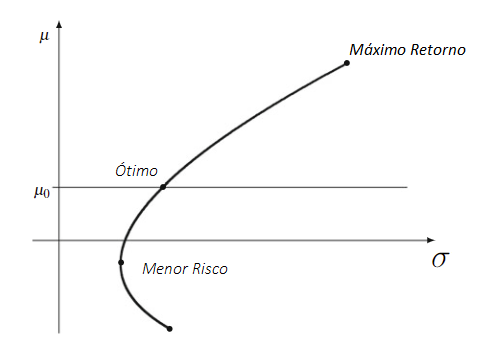
\includegraphics[width=0.6\textwidth]{imagens/minimo_risco.png}
                        \par \footnotesize Fonte: adaptado de \citeonline{mansini2015linear}.
                    \end{figure}

                    \ipar Pela figura, é possível observar uma fronteira que representa todo o conjunto de pontos ótimos para o portfólio, chamada de fronteira eficiente. O ponto ótimo na fronteira eficiente é o ponto de mínimo risco para um determinado nível de retorno.
    
                \paragraph{Índice Sharpe}
                    
                    \ipar O modelo de Média-Variância é um problema de otimização quadrática, pois contém uma função quadrática e restrições lineares. Entretanto, este modelo considera somente um parâmetro para a avaliação do portfólio. Como um investidor pode apresentar diferentes interesses, pode-se adicionar um novo parâmetro para a avaliação do portfólio, a aversão ao risco. 

                    \ipar A aversão ao risco é um parâmetro que representa a preferência do investidor quanto ao risco, e é representado pela letra grega $\lambda$. O modelo de otimização de portfólio com o parâmetro de aversão ao risco é dado por:

                    \begin{equation}
                        \label{eq:aversao}
                        \begin{aligned}
                            & \underset{w}{\text{maximizar}}
                            & & w^T \mu - \lambda w^T \Sigma w \\
                            & \text{sujeito a} \\
                            & & & w^T \mathbf{1} = 1 \\
                            & & & w \geq 0
                        \end{aligned}
                    \end{equation}

                    \ipar Na figura \ref{fig:aversao}, é apresentado um exemplo de otimização de portfólio utilizando o modelo com o parâmetro $\lambda$.

                    \begin{figure}[htbp]
                        \centering
                        \caption{Otimização de portfólio utilizando o modelo com o parâmetro $\lambda$ de aversão ao risco}
                        \label{fig:aversao}
                        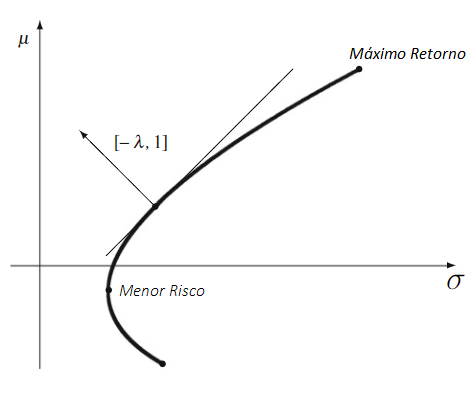
\includegraphics[width=0.6\textwidth]{imagens/aversao.png}
                        \par \footnotesize Fonte: adaptado de \citeonline{mansini2015linear}.
                    \end{figure}

                    \ipar Considerando que existe a opção para o investidor realizar empréstimo ou tomar emprestado a uma taxa livre de risco, é possível construir uma carteira eficiente que combina o empréstimo com todos os investimentos disponíveis no mercado. Esta combinação forma uma linha reta que tangencia a fronteira eficiente de ativos. Esta linha é denominada linha do mercado de capitais, e a carteira eficiente que tangencia a linha é chamada de carteira de mercado, que apresenta o maior prêmio por unidade risco \cite{sharpe1964capital}. A figura \ref{fig:carteira_de_mercado} apresenta um exemplo de linha do mercado de capitais.

                    \begin{figure}[htbp]
                        \centering
                        \caption{Linha do mercado de capitais}
                        \label{fig:carteira_de_mercado}
                        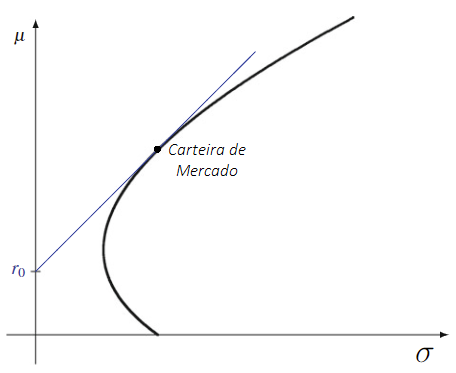
\includegraphics[width=0.6\textwidth]{imagens/carteira_de_mercado.png}
                        \par \footnotesize Fonte: adaptado de \citeonline{mansini2015linear}.
                    \end{figure}

                    \ipar Este modelo de otimização de portfólio é conhecido como modelo de índice de Sharpe, e é dado por:

                    \begin{equation}
                        \label{eq:sharpe}
                        \begin{aligned}
                            & \underset{w}{\text{maximizar}}
                            & & \frac{w^T \mu - r_f}{\sqrt{w^T \Sigma w}} \\
                            & \text{sujeito a} \\
                            & & & w^T \mathbf{1} = 1 \\
                            & & & w \geq 0
                        \end{aligned}
                    \end{equation}

                    \noindent onde $r_f$ é a taxa livre de risco.

                    \ipar O modelo de otimização de portfólio com o Índice Sharpe como função objetivo, é um problema de programação não linear, isto é, contém uma função não linear e restrições lineares. Nas seções seguintes, serão apresentados métodos para resolução de problemas de programação não linear.
                

                    \paragraph{\acrshort{CVaR}}

                  
                    \ipar O Valor em Risco Condicional (\acrshort{CVaR}) é uma medida de risco que busca reduzir a perda de informação dos valores extremos da distribuição. O \acrshort{CVaR} é definido como a média das perdas que excedem o \acrshort{VaR}, ou seja, a média das perdas que excedem o valor máximo de perda que uma carteira de investimentos pode ter em um determinado horizonte de tempo, com uma probabilidade de $1-\alpha$, como apresentado na Figura \ref{fig:CVaR}.
    
    
                    \begin{figure}[htp]
                        \centering
                        \caption{Distribuição da perdas do portfólio, VaR, e CVaR}
                        \label{fig:CVaR}
                        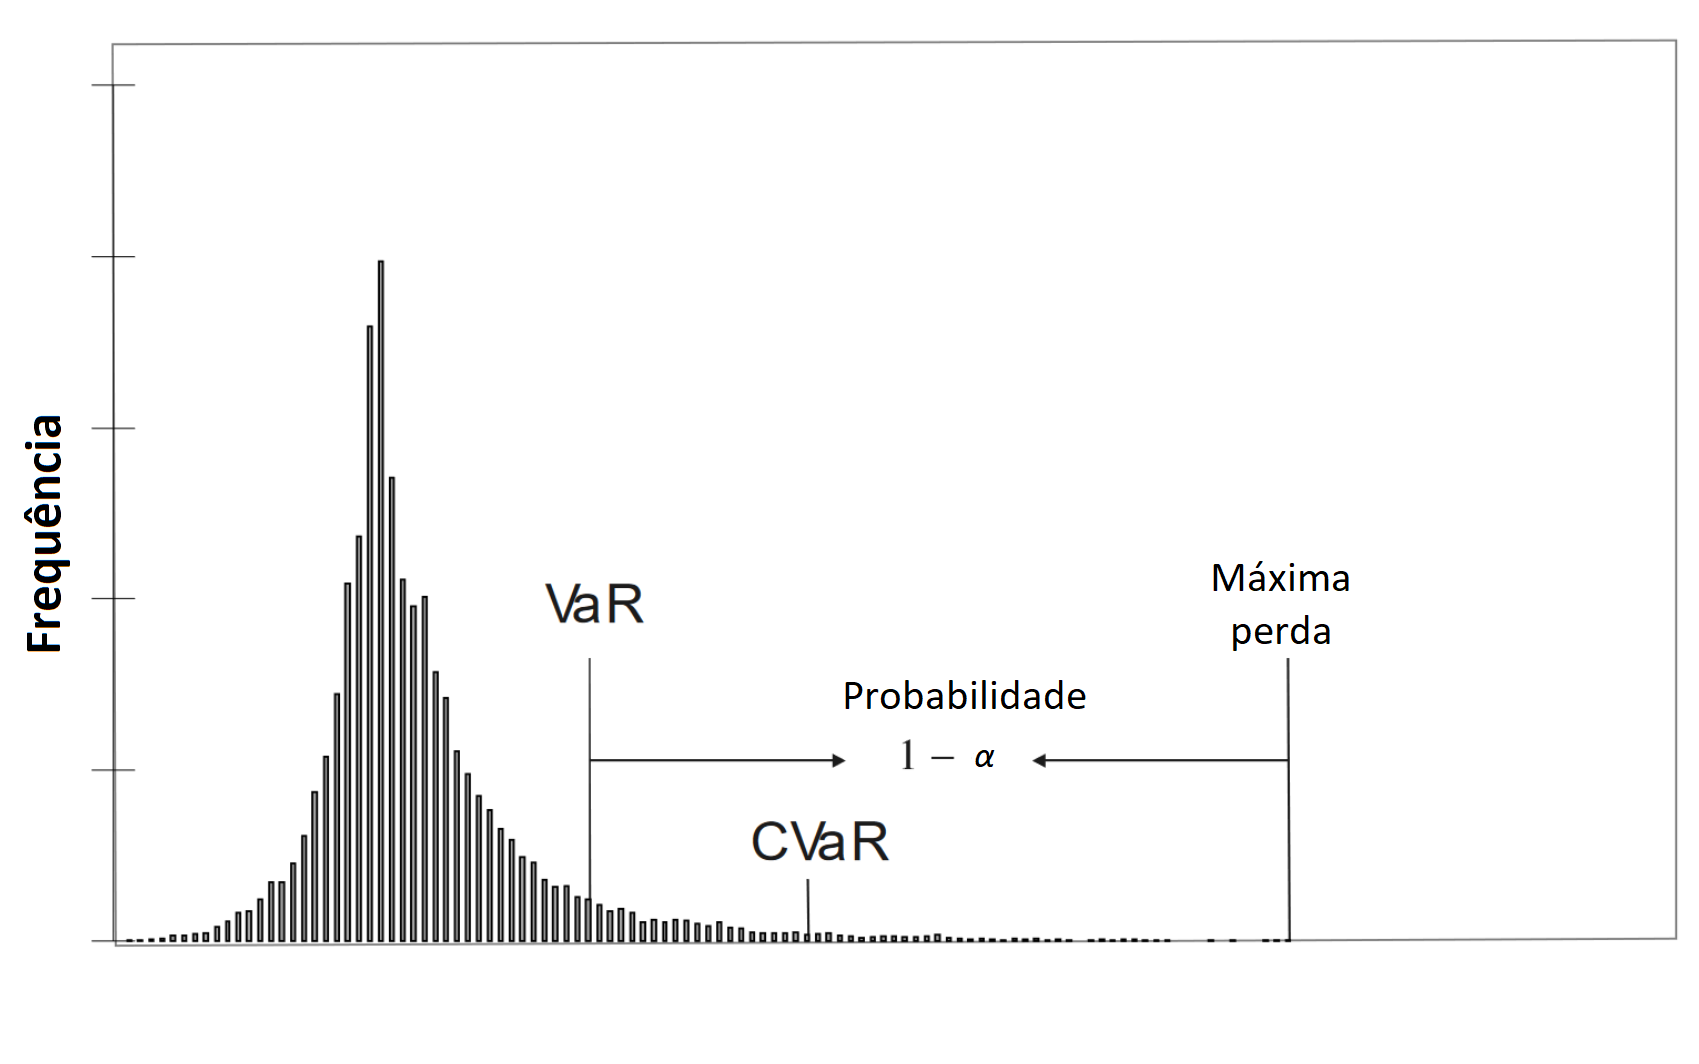
\includegraphics[width=0.7\textwidth]{./imagens/CVaR.png}
                        \par \footnotesize Fonte: adaptado de \citeonline{uryasev2000conditional}.
                    \end{figure}
    
                    Desta maneira, o CVaR pode ser dado como:
    
                    \begin{equation}
                        \label{eq:CVaR}
                        \text{CVaR}_{\beta}(X)=\frac{1}{1-\alpha} \int_{f(X,y)>VaR_{\beta}(X)} f(X,y) p(X) dy,
                    \end{equation}
    
                    \noindent em que $\text{VaR}_{\beta}(X)$ é o valor em risco para um nível de confiança $\beta$, $X$ é a variável de decisão, $y$ é uma variável aleatória que representa o retorno do portfólio, e $p(x)$ é a função de densidade de probabilidade. A fim de simplificar a formulação, \citeonline{uryasev2000conditional} propõe a equação \eqref{eq:f_obj}:

                    \begin{equation}
                        \label{eq:f_obj}
                        F_{\beta}(X,VaR_{\beta}(X))=VaR_{\beta}(X)+\frac{1}{1-\alpha} \int_{f(X,y)>VaR_{\beta}(X)} (f(X,y)-VaR_{\beta}(X)) p(X) dy,
                    \end{equation}

                    \noindent que pode ser utilizada como função objetivo. A função $F_{\beta}(X,VaR_{\beta}(X))$ é uma função convexa, contudo $F_{\beta}(X,VaR_{\beta}(X))$ é definida como uma função linear quando definida no trecho a partir de VaR em $\beta$. O que permite a utilização de métodos de programação linear para o problema. Portanto o problema de otimização de portfólio com o \acrshort{CVaR} como função objetivo pode ser definido como:

                    \begin{equation}
                        \label{eq:CVaR_obj}
                        \begin{aligned}
                            & \underset{w}{\text{minimizar}}
                            & & F_{\beta}(X,VaR_{\beta}(X)) \\
                            & \text{sujeito a} \\
                            & & & z_{t} \geq f(x,y_{t})-VaR_{\beta}(X) \geq 0 \quad \forall t \in \{1, \ldots, n\} \\
                            & & & f(x,y_{t}) = \sum r_{it} x_{i}   \quad \forall t \in \{1, \ldots, n\} \\
                            & & & \mu = \sum \mu_{i} x_{i} \\
                            & & & \mu \geq \mu_0
                        \end{aligned}
                    \end{equation}

                    \noindent onde $z_{t}$ é a diferença entre a média e o retorno do portfólio no instante $t$, $f(x,y_{t})$ é a função de retorno do portfólio no período $t$, $\mu$ é o retorno esperado do portfólio, $\mu_{i}$ é o retorno esperado do ativo $i$, e $\mu_0$ é o retorno esperado mínimo do portfólio.

            \subsubsection{Otimização com parâmetros reais}
            % desenvolvimento da teoria de otimização de portfólio com custos de transação, descrição dos modelos e métodos de otimização aplicados a este problema

                \ipar A utilização de parâmetros reais na otimização busca aproximar o modelo matemático da realidade. A seguir serão apresentados os principais parâmetros reais utilizados na otimização de portfólio.

                \paragraph{Capital de Investimento}
                
                    \ipar A restrição de capital investido permite ao investidor avaliar como o seu capital será alocado entre os ativos. Assim, para esta avaliação, a variável de decisão pode ser modificada para representar a quantidade de capital investido em cada ativo, ao invés da porcentagem de alocação. A restrição de capital investido é dada por:

                    \begin{equation}
                        \begin{aligned}
                            & \sum_{j=1}^{n} x_{j} \leq C_{0} \\
                            & x_{j} \geq 0 \quad j=1, \ldots, n \text{.}
                        \end{aligned}
                    \end{equation}

                    \noindent onde $C_{0}$ é o capital disponível para investimento, e $x_{j}$ é a quantidade de capital investido no ativo $j$. Desta maneira, tanto o retorno do portfólio, quanto o risco e o valor em risco são calculados em valores monetários.
                    
                \paragraph{Custos de operação}

                    \ipar Os custos de operação são compostos por taxas de transação e custos de transação. As taxas de transação são cobradas pelas corretoras e são calculadas em porcentagem do valor negociado. Os custos de transação são calculados em valor monetário e são compostos por taxas de custódia, taxas de liquidação, taxas de emolumentos e taxas de registro. A restrição de custos de operação é dada por:

                    \begin{equation}
                        \begin{aligned}
                        & \sum_{j=1}^{n}\mu_{j}x_{j}- K_{j} = \mu_{0} \sum_{j=1}^{n}x_{j}\\
                        & \sum_{j=1}^{n} x_{j} + K_{j} \leq C_{0} \\
                        & \sum_{j=1}^{n}c_{j}x_{j} + \sum_{j=1}^{n} f_{j} z_{j} = K_{j} \\
                        & x_{j} \leq z_{j} C_{0} \quad j=1, \ldots, n \text{,} \\
                        & x_{j} \geq 0 \quad j=1, \ldots, n \text{,} \\
                        & z_{j} \in\{0,1\} \quad j=1, \ldots, n \\
                        \end{aligned}
                    \end{equation}

                    \noindent onde $c_{j}$ é a taxa de transação do ativo $j$ em porcentagem, $f_{j}$ é o custo de transação do ativo $j$ em valor monetário, $\mu_{j}$ é o retorno esperado do ativo $j$ em valor monetário, $\mu_{0}$ é o retorno esperado do portfólio em valor monetário, $C_{0}$ é o capital disponível para investimento, $x_{j}$ é a quantidade de capital investido no ativo $j$, e $z_{j}$ é uma variável binária que indica se o ativo $j$ está incluído no portfólio ($z_{j}=1$) ou não ($z_{j}=0$), sendo aplicado uma restrição para sua ativação. Assim, o custo da operação também é considerado no cálculo.

                \paragraph{Cotação e Lotes de Negociação}

                    \ipar A cotação e os lotes de negociação são restrições que limitam a quantidade de ativos que podem ser negociados. A cotação é dada em valor monetário e limita o valor mínimo que pode ser negociado. O lote de negociação é dado em quantidade de ativos e limita a quantidade mínima que pode ser negociada. Assim, a variável de decisão se torna a quantidade de lote de cada ativo. A restrição de cotação e lote de negociação é dada por:

                    \begin{equation}
                        \begin{aligned}
                            & x_{j} = \kappa_{j} q_{j} \\
                            &\kappa_{j} \geq 0 \ \in \mathbb{Z} \quad j=1, \ldots, n \\
                        \end{aligned}
                    \end{equation}

                    \noindent onde $x_{j}$ é a quantidade de capital investido no ativo $j$, $\kappa_{j}$ é a quantidade de lotes do ativo $j$, e $q_{j}$ é a cotação do ativo $j$. Com isso, a variável de decisão se torna uma variável inteira. Portanto, necessitando de um método de otimização inteira para sua resolução.
                    
                \paragraph{Rebalanceamento}

                    \ipar O rebalanceamento é uma restrição que permite reinvestir o capital do portfólio. Este capital pode ser combinado com um capital adicional. Também, pode restringir o quanto um ativo será alterado em relação a composição original e avaliar os custos desta operação. Desta maneira, a variável relacionada as taxas de transação é modificada, adicionando uma nova variável para o total de rebalanceamento. A restrição de rebalanceamento é dada por:

                    \begin{equation}
                        \begin{aligned}
                            & \sum_{j=1}^{n}c_{j}q_{j}\delta_{j} + \sum_{j=1}^{n} f_{j} z_{j}  = K_{j} \\
                            & C_{0} = \sum_{i=1}^{n}q_{i}\kappa_{i}^{0}+ B \\
                            & \delta_{j} \geq \left( \kappa_{j} -\kappa_{j}^{0} \right) \quad j=1, \ldots, n\\
                            & \delta_{j} \geq -\left( \kappa_{j} -\kappa_{j}^{0} \right) \quad j=1, \ldots, n\\
                            & \delta_{j} \leq \gamma_{j}z_{j} \quad j=1, \ldots, n\\
                            & \delta_{j} \geq 0 \ \in \mathbb{Z} \quad j=1, \ldots, n\\
                            & z_{j} \in\{0,1\} \quad j=1, \ldots, n \\
                        \end{aligned}
                    \end{equation}

                    \noindent onde $c_{j}$ é a taxa de transação do ativo $j$ em porcentagem, $f_{j}$ é o custo de transação do ativo $j$ em valor monetário, $q_{j}$ é a cotação do ativo $j$, $\kappa_{j}$ é a quantidade de lotes do ativo $j$, $\kappa_{j}^{0}$ é a quantidade de lotes do ativo $j$ no portfólio original, $B$ é o capital adicional, $C_{0}$ é o capital disponível para investimento, $\delta_{j}$ é a quantidade de lotes do ativo $j$ que será alterado, e $z_{j}$ é modificado, sendo é uma variável binária que indica se o ativo $j$ está sendo rebalanceado no portfólio ($z_{j}=1$) ou não ($z_{j}=0$), e $\gamma_{j}$ é quantidade limite de alteração de lotes do ativo j. Assim, o custo da operação também é considerado no cálculo.


                \paragraph{Cardinialidade}

                    \ipar A cardinalidade é uma restrição que limita o número de ativos que podem ser incluídos no portfólio. A restrição de cardinalidade pode ser expressa matematicamente da seguinte forma:

                    \begin{equation}
                        \begin{aligned}
                            & \sum_{j=1}^{n} a_{j} \leq N \\
                            &\kappa_{j} q_{j} \leq a_{j} C_{0} \quad j=1, \ldots, n \\
                            & a_{j} \in\{0,1\} \quad j=1, \ldots, n \\
                        \end{aligned}
                    \end{equation}

                    \noindent onde $a_{j}$ é uma variável binária que indica se o ativo $j$ está incluído no portfólio ($a_{j}=1$) ou não ($a_{j}=0$), $n$ é o número total de ativos e $N$ é o número máximo de ativos que podem ser incluídos no portfólio. Uma restrição adicional é necessária para a ativação da variável binária $a_{j}$.
                    
                \paragraph{Aversão ao Risco}

                    \ipar A aversão ao risco é uma variável que permite ao investidor controlar o nível de exposição ao risco do portfólio. A pergunta que esta restrição responde é: quanto está disposto a perder para obter um retorno maior? Considerando que o investidor é capaz de realizar um empréstimo a juros. A restrição de aversão ao risco é dada por:
                    
                    \begin{equation}
                        \begin{aligned}
                            & \mu_{p} - \sigma_{p} Z_\beta \geq VaR \\
                        \end{aligned}
                    \end{equation}

                    \noindent onde $\mu_{p}$ é o retorno esperado da carteira, $\sigma_{p}$ é o risco da carteira, $Z_\beta$ é o valor multiplicador do desvio padrão dado nível de confiança, e $VaR$ é o valor monetário de risco de perda aceitável da carteira.

            \subsubsection{Métodos de Otimização}

                \ipar A otimização de carteira de investimentos pelo índice Sharpe é um problema de otimi-zação não linear. Assim ferramentas de otimização não linear podem ser utilizadas para resolver o problema. Além disso, o problema quando incorpora parâmetros reais, inclui variáveis inteiras, e este tipo de problema é conhecido como problema de otimização misto inteiro, que demandam métodos de otimização específicos. A seguir são apresentados alguns métodos de otimização que podem ser utilizados para resolver o problema de otimização de carteira de investimentos.

                \ipar \citeonline{kraft1988sqlsp} desenvolveu o método de Programação Quadrática (\acrshort{SLSQP}, do inglês \textit{Sequencial Sequential Least Squares Programming}) que é um método para resolução de problemas de otimização não linear. O \acrshort{SLSQP} é iterativo e resolve problemas de otimização não linear com restrições de igualdade e desigualdade. O método é de segunda ordem, isto é, utiliza a matriz Hessiana da função objetivo para determinar a direção de busca, e aplica a método do conjunto ativo na realização dos cálculos. Por ser um método de programação não linear, o \acrshort{SLSQP} não é capaz de resolver problemas de otimização misto inteiro, sendo assim necessário a utilização de métodos de otimização misto inteiro.

                \ipar A resolução de problemas de otimização inteira, como os problemas de seleção de ativos para portfólios que consideram restrições reais, necessitam de métodos para a ordenação da resolução. Métodos para otimização inteira são \textit{Branch-and-Bound}, \textit{Branch-and-Cut}. O \textit{Branch-and-Bound} é um método de otimização inteira que utiliza a técnica de divisão e conquista para resolver problemas de otimização inteira. O método consiste em dividir o problema em subproblemas, e resolver cada subproblema de forma recursiva. O \textit{Branch-and-Cut} é um método de otimização inteira que utiliza o \textit{Branch-and-Bound} e cortes para resolver problemas de otimização inteira.

                \ipar \citeonline{hedengren2014nonlinear} desenvolveu um método para resolução de problemas de progamação não linear inteira mista no qual combina o método \acrshort{SLSQP} com o método \textit{Branch-and-Bound}. Este método é chamado de \textit{APOPT}, do inglês \textit{Advanved Process Optimization with Partial Integer Programming Technology}. O \textit{APOPT} é um método de otimização não linear inteira mista que utiliza o \acrshort{SLSQP} para resolver problemas de otimização não linear e o \textit{Branch-and-Bound} para resolver problemas de otimização inteira. O \textit{APOPT} é capaz de resolver problemas de otimização não linear inteira mista com restrições de igualdade e desigualdade.


            \subsubsection{Heurística}

                \ipar A aplicação de restrições reais no problema de otimização, como a taxa de transação, limitação de capital, e restrições como a de cardinalidade, e outros, aumenta a complexidade do problema. Otimização de carteira de investimentos com restrições reais é considerado um problema NP-difícil, isto é, um problema não polinomial de difícil resolução \cite{milhomem2020analysis}. Uma abordagem para resolução de problemas complexos é a utilização de métodos heurísticos, que são métodos de busca que não garantem a solução ótima, mas são capazes de encontrar soluções próximas da ótima em um tempo computacionalmente viável.


                % \paragraph{Matheurística de Busca Básica no Núcleo}
        
                    \ipar Após \citeonline{angelelli2008comparison} avaliarem modelos de otimização com parâmetros reais, como custo de transação, disponibilidade de capital, limites de quantidades além de realizar otimização por programação linear inteira mista, conclue-se que a otimização por programação linear inteira mista para modelo de CVaR exige um alto tempo computacional, especialmente quando há uma grande quantidade de parâmetros no modelo, como mais de 200 ativos. No entanto, também foi observado que modelos heurísticos obtém resultados satisfatórios em um tempo computacional menor.
                
                    \ipar Assim propuseram uma matheurística, uma heurística que transforma as variáveis discretas em variáveis contínuas para escolha inicial de ativos para o núcleo que posteriormente são combinados com pequenas parcelas dos ativos restantes para realizar a otimização por programação inteira mista, este modelo é chamado de busca básica no núcleo (do inglês, \textit{Basic Kernel Search} - BKS). O modelo de busca básica do núcleo elaborado por \citeonline{angelelli2012kernel} está descrito no Algoritmo \ref{alg:BKS}.
                
                    \begin{algorithm}
                        \floatname{algorithm}{Algoritmo}
                        \caption{Esquema geral da Busca Básica do Núcleo}
                        \label{alg:BKS}
                        1. Identificar o núcleo inicial e organizar os demais ativos em parcelas de listas ordenadas. \\
                        2. Resolver o problema de otimização inteira mista restrito ao núcleo inicial. \\
                        3. Enquanto critério de parada não é atingido. \\
                            (a) Adicionar próxima parcela de ativos ao núcleo, formado um único conjunto; \\
                            (b) Resolver o problema de otimização inteira mista para o conjunto formado; \\
                            (c) Remover do conjunto os ativos não escolhidos da parcela adicional e adicionar os escolhidos ao núcleo. 
                        \par \footnotesize Fonte: adaptado de \citeonline{mansini2015linear}. % Fonte: \citeonline{Autor_bibtex}.
                        \end{algorithm}
                
                    \ipar Na etapa 1, as variáveis discretas são transformadas em variáveis contínuas e aplica-se a otimização. Com a solução da etapa 1, a parcela do núcleo, que geralmente não é superior a 100 ativos de acordo com \citeonline{mansini2015linear}, é separada e os demais ativos são ordenados utilizando um critério de preferência. Então, os ativos fora do núcleo são divididos em parcelas de até $l$ quantidades, formando conjuntos $\{B_i\}$, como representado na Figura \ref{fig:parcelas}. 
                
                    \begin{figure}[H]
                        \centering
                        \caption{Organização dos ativos na Busca Básica do Núcleo}
                        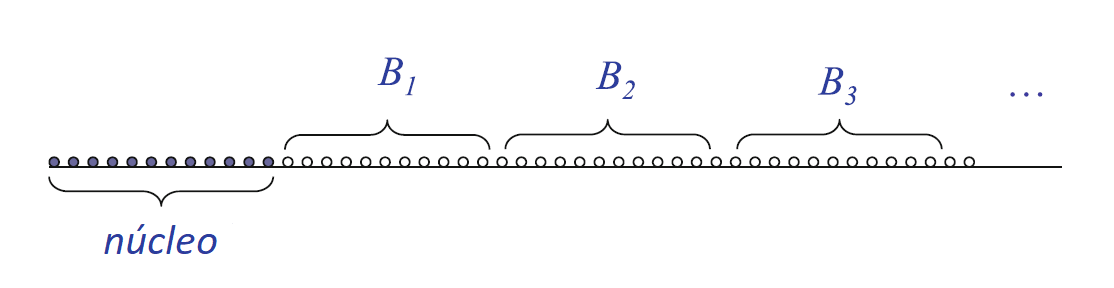
\includegraphics[width=0.6\textwidth]{imagens/parcelas.png}
                        \label{fig:parcelas}
                        \par \footnotesize Fonte: adaptado de \citeonline{mansini2015linear}. % Fonte: \citeonline{Autor_bibtex}.
                    \end{figure}
                
                    \ipar Na etapa 2, o modelo de programação linear inteira mista é resolvido com o núcleo de ativos inicial, e caso não haja solução, o resultado é definido como $-\infty$. Na etapa 3, adiciona-se duas restrições, uma que ao menos um ativo do conjunto $B_i$ deve ser escolhido e outra que a solução obtida na etapa 2 deve ser melhorada. Caso a etapa 3.a seja viável, o modelo de programação linear inteira mista segue para a próxima etapa. Entretanto, tem-se o critério de parada se a solução para a etapa 3.b for inviável. Portanto, o modelo heurístico busca reduzir o problema de otimização inteira mista para uma parcela menor e com menor custo computacional. 

                    \ipar Este algoritmo pode aplicar como critério de ordenação o de maior índice de Sortino. Este índice é dado pelo retorno do portfólio dividido pelo desvio padrão dos retornos negativos do ativo. Para este trabalho, utilizaremos o índice de Sharpe.
       
    \subsection{REDES NEURAIS ARTIFICIAIS}
        \label{sec:redesneurais}
        % Apresentação dos modelos de previsão de retorno de ativos, redes neurais, redes neurais recorrentes

        Nesta seção, serão apresentados modelos de redes neurais artificiais. As redes neurais são modelos computacionais inspirados no funcionamento do cérebro humano, capazes de aprender e realizar tarefas complexas de processamento de informações. Serão abordadas as redes neurais artificiais, redes neurais recorrentes, mecanismo de atenção e otimização hiperparâmetros.
        
        \ipar As redes neurais artificiais, também conhecidas como perceptrons multicamadas, são o tipo mais comum de redes neurais utilizadas na previsão de retornos de ativos. Essas redes são compostas por várias camadas de neurônios, em que cada neurônio de uma camada está conectado a todos os neurônios da camada seguinte. A informação flui apenas em uma direção, da entrada para a saída, sem feedback ou ciclos na rede. Essas redes são treinadas por meio do algoritmo de retropropagação do erro, que ajusta os pesos das conexões para minimizar a diferença entre os valores de saída esperados e os valores de saída previstos.

        \ipar As redes neurais artificiais são capazes de aprender relações não lineares entre as variáveis de entrada e saída, o que as torna adequadas para a previsão de retornos de ativos financeiros. Entretanto, essas redes apresentam problemas com o sobreajuste, que ocorre quando a rede aprende os dados de treinamento muito bem, mas não consegue generalizar para novos dados. Para resolver esse problema, foram propostas as redes neurais recorrentes, que são capazes de aprender dependências de longo prazo e são amplamente utilizadas na previsão de séries temporais financeiras.

        \subsubsection{Redes Neurais Recorrentes}
        
            \ipar As redes neurais recorrentes são um tipo especial de rede neural que possui conexões retroalimentadas, permitindo que informações do passado sejam incorporadas na previsão do futuro. Isso as torna adequadas para a previsão de séries temporais, como os retornos de ativos financeiros. As \acrshort{RNN} apresentam problemas com a perda do gradiente, que ocorre quando o gradiente de erro se torna muito pequeno, fazendo com que a rede pare de aprender. Para resolver esse problema, foram propostas as redes neurais recorrentes de memória de curto prazo (\acrshort{LSTM}) e as redes neurais recorrentes de memória de longo prazo (\acrshort{GRU}).

            \ipar A rede \acrshort{LSTM} é um tipo de rede recorrente que possui blocos de memória (células) na camada oculta que são conectados de forma recorrente. Existem dois estados que são transferidos para a próxima célula: o estado da célula e o estado oculto. Os blocos de memória são responsáveis por lembrar as informações, e as manipulações dessa memória são feitas por meio de três mecanismos principais chamados de portões. Um portão de esquecimento é responsável por remover informações do estado da célula. O portão de entrada é responsável pela adição de informações ao estado da célula. O portão de saída decide qual próximo estado oculto deve ser selecionado. A Figura \ref{fig:lstm} ilustra como o cálculo é realizado em uma célula \acrshort{LSTM}.

            \begin{figure}[htbp]
                \centering
                \caption{Célula LSTM.}
                \label{fig:lstm}
                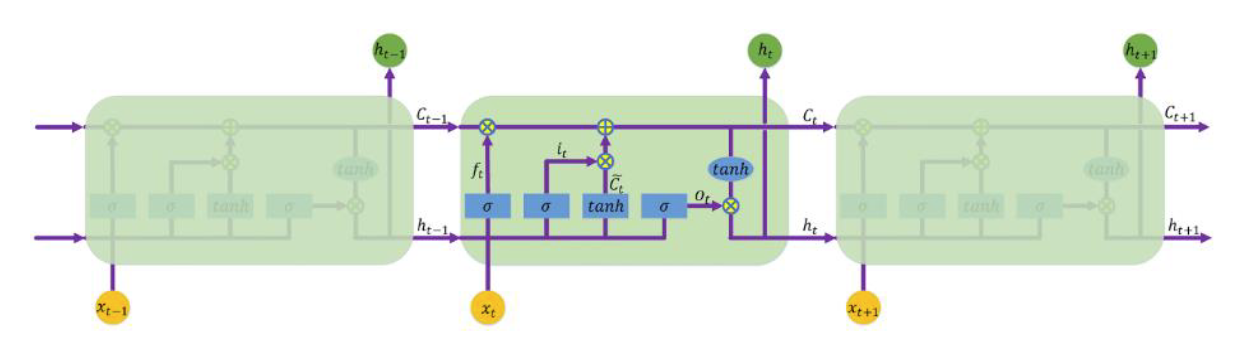
\includegraphics[width=0.95\textwidth]{imagens/lstm.png}
                \par \footnotesize Fonte: \citeonline{ta2020portfolio}.
            \end{figure}


            \ipar As operações realizadas nas unidades da rede \acrshort{LSTM} são explicadas em \eqref{eq:lstm}, onde $x_t$ é a entrada no tempo $t$ e $f_t$ é o portão de esquecimento no tempo $t$, que limpa as informações da célula de memória quando necessário e mantém um registro do quadro anterior cuja informação precisa ser apagada da memória. O portão de saída $o_t$ mantém as informações sobre a etapa seguinte, onde $g$ é a unidade recorrente, tendo a função de ativação "tanh", e é calculado a partir da entrada do quadro atual e do estado do quadro anterior $h_{t-1}$. Em todos os portões de entrada ($I_t$), esquecimento ($f_t$) e saída ($o_t$), bem como na unidade recorrente ($g_t$), usamos ($W_i$, $W_f$, $W_o$, $W_g$) e ($b_i$, $b_f$, $b_o$, $b_g$) como pesos e viés, respectivamente. O portão de entrada determina quais partes da entrada transformada $g_t$ precisam ser adicionadas ao estado de longo prazo $c_t$. Esse processo atualiza o estado de longo prazo $c_t$, que é transmitido diretamente para a próxima célula. Finalmente, o portão de saída transforma o estado de longo prazo atualizado $c_t$ através de $tanh(.)$; filtra-o por $o_t$; e produz a saída $y_t$, que também é enviada para a próxima célula como o estado de curto prazo $h_t$.

            \begin{equation}
                \label{eq:lstm}
                \begin{aligned}
                    & f_t = \sigma(W_f \cdot [h_{t-1}, x_t] + b_f) \\
                    & i_t = \sigma(W_i \cdot [h_{t-1}, x_t] + b_i) \\
                    & o_t = \sigma(W_o \cdot [h_{t-1}, x_t] + b_o) \\
                    & g_t = \tanh(W_g \cdot [h_{t-1}, x_t] + b_g) \\
                    & c_t = f_t \cdot c_{t-1} + i_t \cdot g_t \\
                    & h_t = o_t \cdot \tanh(c_t) \\
                \end{aligned}
            \end{equation}

            \noindent onde $\sigma(.)$ é a função logística e $\tanh(.)$ é a função tangente hiperbólica. Os três portões abrem e fecham de acordo com o valor dos controladores de portão $f_t$, $i_t$ e $o_t$, todos os quais são camadas totalmente conectadas de neurônios. A faixa de suas saídas é [0, 1], pois eles usam a função logística para ativação. Em cada portão, suas saídas são alimentadas em operações de multiplicação elemento a elemento, então, se a saída estiver próxima de 0, o portão é estreitado e menos memória é armazenada em $c_t$, enquanto se a saída estiver próxima de 1, o portão está mais aberto, deixando mais memória fluir através do portão. Dadas as células \acrshort{LSTM}, é comum empilhar várias camadas das células para tornar o modelo mais profundo para ser capaz de capturar a não linearidade dos dados. 

            \ipar Nas redes \acrshort{GRU}, a estrutura é semelhante à das redes \acrshort{LSTM}, mas com menos parâme-tros. A principal diferença entre as redes \acrshort{LSTM} e \acrshort{GRU} é que as redes \acrshort{GRU} não possuem uma célula de memória separada e, portanto, não possuem um estado de célula. Em vez disso, elas possuem um estado oculto único que é usado para controlar o fluxo de informações. As redes \acrshort{GRU} também possuem apenas dois portões: um portão de atualização e um portão de reinicialização. O portão de atualização decide quanta informação do passado deve ser mantida no estado oculto atual. O portão de reinicialização decide quanta informação do passado deve ser esquecida. A saída da célula \acrshort{GRU} é calculada a partir do estado oculto atual e da entrada atual. A saída da célula \acrshort{GRU} é então passada para a próxima célula como o estado oculto. Assim, as redes \acrshort{GRU} são mais simples do que as redes \acrshort{LSTM}, mas ainda são capazes de capturar dependências de longo prazo nas séries temporais de retorno de ativos.
        
        \subsubsection{Mecanismo de Atenção}
        
            \ipar Apesar de sua eficácia em aprender padrões localizados no tempo, as redes \acrshort{LSTM} têm dificuldade em capturar dependências significativas quando o comprimento de uma sequência é relativamente grande. O mecanismo de atenção foi desenvolvido para resolver esse problema e agora foi estabelecida como estado da arte na maioria dos trabalhos em processamento de linguagem natural. Vários estudos também mostram a aplicação bem-sucedida dessa arquitetura no domínio financeiro.             
            
            \ipar No centro de toda arquitetura está um mecanismo chamado de atenção, e é dado por:

            \begin{equation}
                \label{eq:attention}
                \begin{aligned}
                    & \text{Attention}(Q, K, V) = \text{softmax}\left(\frac{QK^T}{\sqrt{d_k}}\right)V \\
                \end{aligned}
            \end{equation}
        
            \ipar A matriz de valor $V \in \mathbb{R}^{\tau \times d_v}$ da equação \ref{eq:attention} é ponderada por um conjunto de pontuações obtidas pela operação \textit{softmax}, que determina quanta ênfase cada etapa da matriz de chaves $K \in \mathbb{R}^{\tau \times d_k}$ deve receber ao codificar posições de sequência da matriz de consultas $Q \in \mathbb{R}^{\tau \times d_k}$. O produto escalar de $Q$ e $K$ é dividido pela raiz quadrada da dimensão de codificação ($d_{model}$) para evitar problemas associados a pequenos gradientes. Além disso, o mecanismo de atenção implementa uma máscara por meio da matriz $M \in \mathbb{R}^{\tau \times \tau}$ no primeiro bloco de atenção de cada camada do decodificador para garantir que ele só possa atender às etapas de tempo anteriores e, portanto, manter sua propriedade autorregressiva. Os modelos que utilizam as consultas e as chaves de atenção são chamados de \textit{self-attention} e são capazes de capturar dependências de longo alcance em uma sequência. A figura \ref{fig:attention} ilustra o mecanismo de atenção.

            \begin{figure}[H]
                \centering
                \caption{Mecanismo de atenção.}
                \label{fig:attention}
                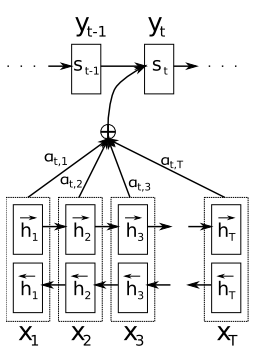
\includegraphics[width=0.3\textwidth]{imagens/attention.png}
                \par \footnotesize Fonte: \citeonline{bahdanau2015neural}.
            \end{figure}

            \ipar A figura \ref{fig:attention} ilustra um modelo de atenção que tenta gerar a palavra alvo $y_t$ dada uma sentença de origem $x_1, x_2, \dots, x_T$. O modelo de atenção é capaz de capturar dependências de longo alcance entre origem e destino.

        \subsubsection{Otimização de hiperparâmetros}

            \ipar O desempenho de algoritmos de redes neurais dependem de uma série de hiperparâme-tros, como o número de camadas, o número de neurônios por camada, a taxa de aprendizado, o tamanho do lote de treinamento, entre outros. A busca de hiperparâmetros é um processo demorado e caro, pois envolve a avaliação de várias configurações de hiperparâmetros. A maioria dos algoritmos de otimização de hiperparâmetros é baseada em métodos de busca aleatória. Esses métodos de busca aleatória são ineficientes, pois não levam em consideração o desempenho de configurações anteriores. Além disso, eles não são capazes de explorar regiões promissoras do espaço de hiperparâmetros. Assim, uma alternativa é a utilização de um método estruturado de busca de hiperparâmetros, como o HyperBand.

            \ipar O HyperBand é um algoritmo de otimização de hiperparâmetros que foi proposto por \citeonline{li2018hyperband} para acelerar o processo de busca de hiperparâmetros. Ele utiliza um método de busca aleatória para explorar o espaço de hiperparâmetros e um método de busca em largura para explorar regiões promissoras. Na figura \ref{fig:hyperband} é ilustrado o algoritmo HyperBand.

            \begin{figure}[htbp]
                \centering
                \caption{Algoritmo HyperBand.}
                \label{fig:hyperband}
                \begin{subfigure}{.5\textwidth}
                    \centering
                    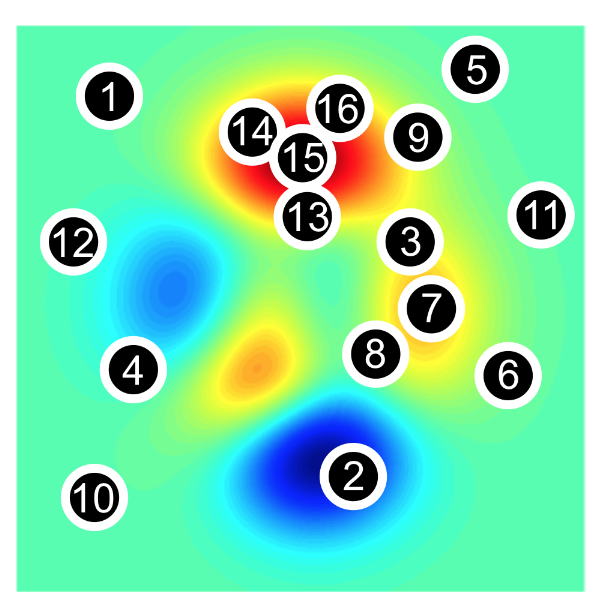
\includegraphics[width=.7\linewidth]{imagens/configuration_selection.png}
                    \caption{Configuração de seleção.}
                    \label{fig:hyperband_configuration}
                    % \par \footnotesize Fonte: próprio autor.
                \end{subfigure}%
                \begin{subfigure}{.5\textwidth}
                    \centering
                    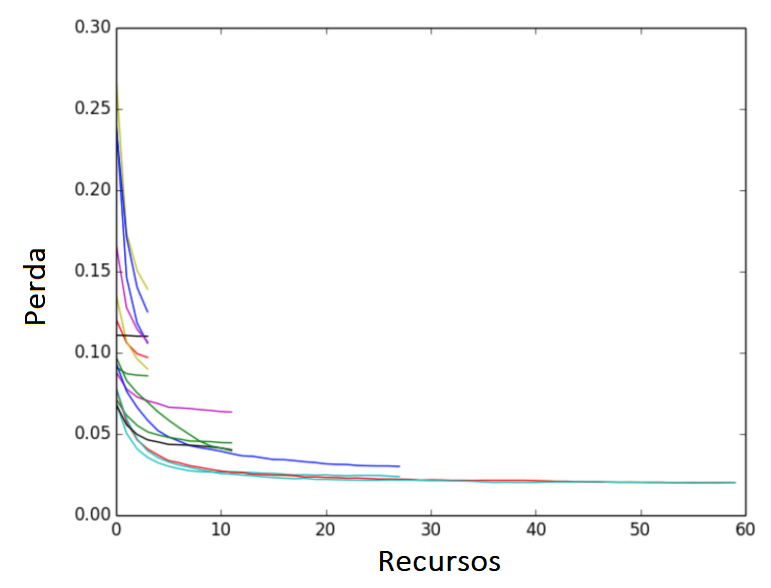
\includegraphics[width=.95\linewidth]{imagens/configuration_evaluation.png}
                    \caption{Configuração de avaliação.}
                    \label{fig:hyperband_evaluation}
                \end{subfigure}
                \par \footnotesize Fonte: adaptado de \cite{li2018hyperband}.
            \end{figure}

            % Figure 1: (a) The heatmap shows the validation error over a two-dimensional search space with red corresponding to areas with lower validation error. Configuration selection methods adaptively choose new configurations to train, proceeding in a sequential manner as indicated by the numbers. 

            \ipar O algoritmo HyperBand é composto por duas etapas: seleção de configuração e avaliação de configuração. Na etapa de configuração, o algoritmo seleciona aleatoriamente uma configuração de hiperparâmetros e treina o modelo com essa configuração por um número fixo de épocas. A figura \ref{fig:hyperband_configuration} ilustra a etapa de seleção de configuração, no qual o mapa de calor mostra o erro de validação sobre um espaço de busca bidimensional com a cor vermelho correspondendo a áreas com menor erro de validação. O método seleciona de forma adaptativa novas configurações para treinar, procedendo de forma sequencial como indicado pelas numerações.
            
            % (b) The plot shows the validation error as a function of the resources allocated to each configuration (i.e. each line in the plot). Configuration evaluation methods allocate more resources to promising

            \ipar Na etapa de avaliação, o algoritmo avalia a configuração e seleciona os modelos mais promissores. A figura \ref{fig:hyperband_evaluation} ilustra a etapa de avaliação de configuração, na qual o gráfico mostra o erro de validação como uma função dos recursos alocados para cada configuração, ou seja, cada linha no gráfico. Os métodos de avaliação de configuração alocam mais recursos para configurações promissoras.

\pagebreak